\documentclass[12pt, a4paper]{article}

\usepackage[utf8]{inputenc}
\usepackage[T1]{fontenc}
\usepackage[brazil]{babel}
\usepackage{lmodern}
\usepackage{geometry}
\usepackage{graphicx}
\usepackage{booktabs}
\usepackage{array}
\usepackage{amsmath}
\usepackage{float}
\usepackage{caption}
\usepackage{indentfirst}
\usepackage{setspace}
\usepackage{parskip}

\geometry{top=2.5cm, bottom=2.5cm, left=3cm, right=2.5cm}
\setlength{\parskip}{6pt}

\graphicspath{{../output-cifar-10/}}

\title{\large\textbf{Simulação de Aprendizado Federado: Novos Experimentos}}
\author{Júlio}
\date{\today}

% ═════════════════════════════════════════════════
\begin{document}

\maketitle

Este relatório apresenta os resultados dos três estudos conduzidos após a entrega
inicial: (i) estudo de ablação do fator de agregação assíncrono (CIFAR-10);
(ii) generalização para múltiplos datasets; e (iii) análise do impacto do
\textit{timeout} no cenário síncrono (CIFAR-10).

% ─────────────────────────────────────────────
\section{Datasets Utilizados}

Os experimentos de generalização avaliaram quatro datasets com complexidades distintas,
conforme a Tabela~\ref{tab:datasets}.

\begin{table}[H]
\centering
\caption{Datasets avaliados nos experimentos de generalização.}
\label{tab:datasets}
\renewcommand{\arraystretch}{1.25}
\begin{tabular}{llcc}
\toprule
\textbf{Dataset} & \textbf{Tarefa} & \textbf{Classes} & \textbf{Complexidade} \\
\midrule
MNIST        & Dígitos manuscritos      & 10 & Baixa       \\
Fashion MNIST & Peças de roupa          & 10 & Média-baixa \\
CIFAR-10     & Objetos naturais (RGB)   & 10 & Média-alta  \\
GTSRB        & Placas de trânsito (RGB) & 43 & Alta        \\
\bottomrule
\end{tabular}
\end{table}

A distribuição dos dados entre clientes foi avaliada em dois cenários —
\textbf{IID} e \textbf{Não-IID} — conforme descrito no relatório anterior.

% ─────────────────────────────────────────────
\section{Configuração Experimental}

\begin{table}[H]
\centering
\caption{Parâmetros utilizados nos experimentos.}
\label{tab:params}
\renewcommand{\arraystretch}{1.25}
\begin{tabular}{lcc}
\toprule
\textbf{Parâmetro} & \textbf{Ablação / Generalização} & \textbf{Impacto do Timeout} \\
\midrule
Modo                                   & Assíncrono            & Síncrono              \\
Dataset                                & CIFAR-10 / múltiplos  & CIFAR-10              \\
Número de clientes                     & 40                    & 40                    \\
Rodadas / atualizações                 & 40 / 80               & 80                    \\
Épocas locais por rodada               & 1                     & 1                     \\
\textit{Batch size}                    & 32                    & 32                    \\
Atraso de conexão                      & $\mathcal{U}(0,5)$ s  & $\mathcal{U}(0,5)$ s  \\
Atraso de treinamento                  & $\mathcal{U}(0,90)$ s & $\mathcal{U}(0,90)$ s \\
Probabilidade de conexão               & $p50$                 & —                     \\
Fator base $\alpha_0$                  & 0{,}3 / 0{,}5 / 0{,}8 (ablação) & —           \\
Decaimento $\delta$                    & 0{,}95 / 0{,}99 / 0{,}999 (ablação) & —       \\
Sensibilidade $\lambda$                   & 0 / 0{,}075 / 0{,}5 (ablação) & —             \\
Timeout (percentil via Monte Carlo)    & —                     & P25 / P50 / P75 / Sem \\
Semente aleatória                      & 42                    & 42                    \\
\bottomrule
\end{tabular}
\end{table}

Para o estudo de impacto do \textit{timeout}, os valores foram derivados via simulação
de Monte Carlo ($10^6$ realizações de $\Delta t = \Delta t_{\text{conn}} + \Delta t_{\text{train}}$),
obtendo os percentis $P_{25} = 24{,}99$ s, $P_{50} = 47{,}45$ s, $P_{75} = 69{,}95$ s
e o limite máximo de $95{,}00$ s (sem timeout).

% ─────────────────────────────────────────────
\section{Estudo de Ablação — FL Assíncrono (CIFAR-10)}

Foram conduzidos 14 experimentos \textit{one-at-a-time}, variando isoladamente
cada parâmetro do fator de agregação
$\gamma_t = \alpha_0 \cdot \delta^{v_t} \cdot (1 + \lambda\, \tau_t)^{-1}$.
As demais variáveis foram mantidas fixas nos valores padrão:
$\alpha_0 = 0{,}8$, $\delta = 0{,}999$, $\lambda = 0{,}075$.

\subsection{Impacto do Fator Base $\alpha_0$}

\begin{table}[H]
\centering
\caption{Impacto de $\alpha_0$ na acurácia. Fixos: $\delta=0{,}999$, $\lambda=0{,}075$.}
\label{tab:alpha}
\renewcommand{\arraystretch}{1.25}
\resizebox{\textwidth}{!}{%
\begin{tabular}{cccccc}
\toprule
$\alpha_0$ & IID máx. & IID avg\_last10 & Non-IID máx. & Non-IID avg\_last10 & Non-IID tail\_std \\
\midrule
0{,}3 & 0{,}6578          & 0{,}6569          & \textbf{0{,}4609} & \textbf{0{,}4350} & 0{,}0329          \\
0{,}5 & 0{,}6785          & 0{,}6771          & 0{,}4581          & 0{,}3857          & 0{,}0435          \\
0{,}8 & \textbf{0{,}6812} & \textbf{0{,}6800} & 0{,}4604          & 0{,}3760          & \textbf{0{,}0588} \\
\bottomrule
\end{tabular}}
\end{table}

Em IID, o impacto de $\alpha_0$ é pequeno ($\approx 2\%$). Em Non-IID, $\alpha_0 = 0{,}8$
apresenta o dobro do desvio-padrão de $\alpha_0 = 0{,}3$ na cauda ($0{,}059$ vs $0{,}033$):
valores altos amplificam as oscilações causadas por updates heterogêneos.

\begin{figure}[H]
    \centering
    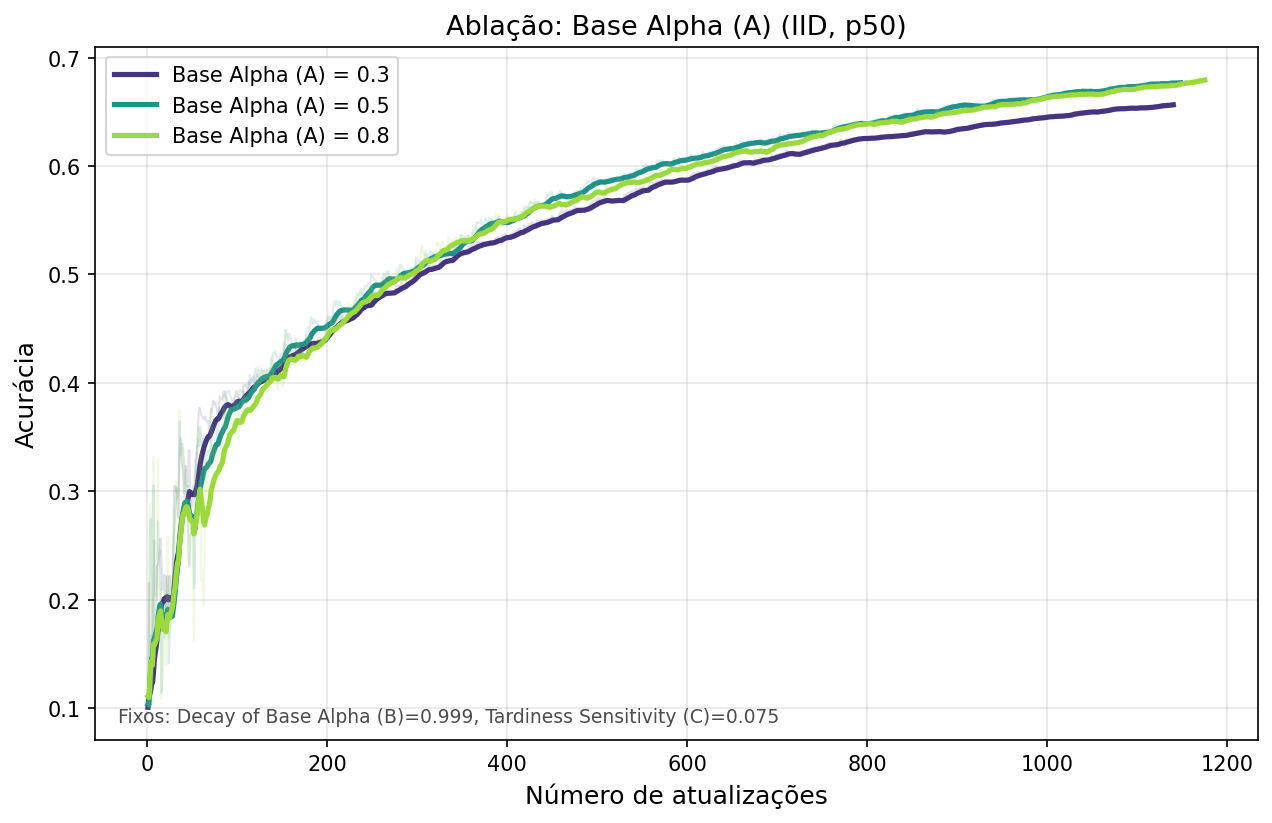
\includegraphics[width=\textwidth]{ablation_base_alpha_iid_p50.png}
    \caption{Ablação de $\alpha_0$ — cenário IID.}
\end{figure}

\begin{figure}[H]
    \centering
    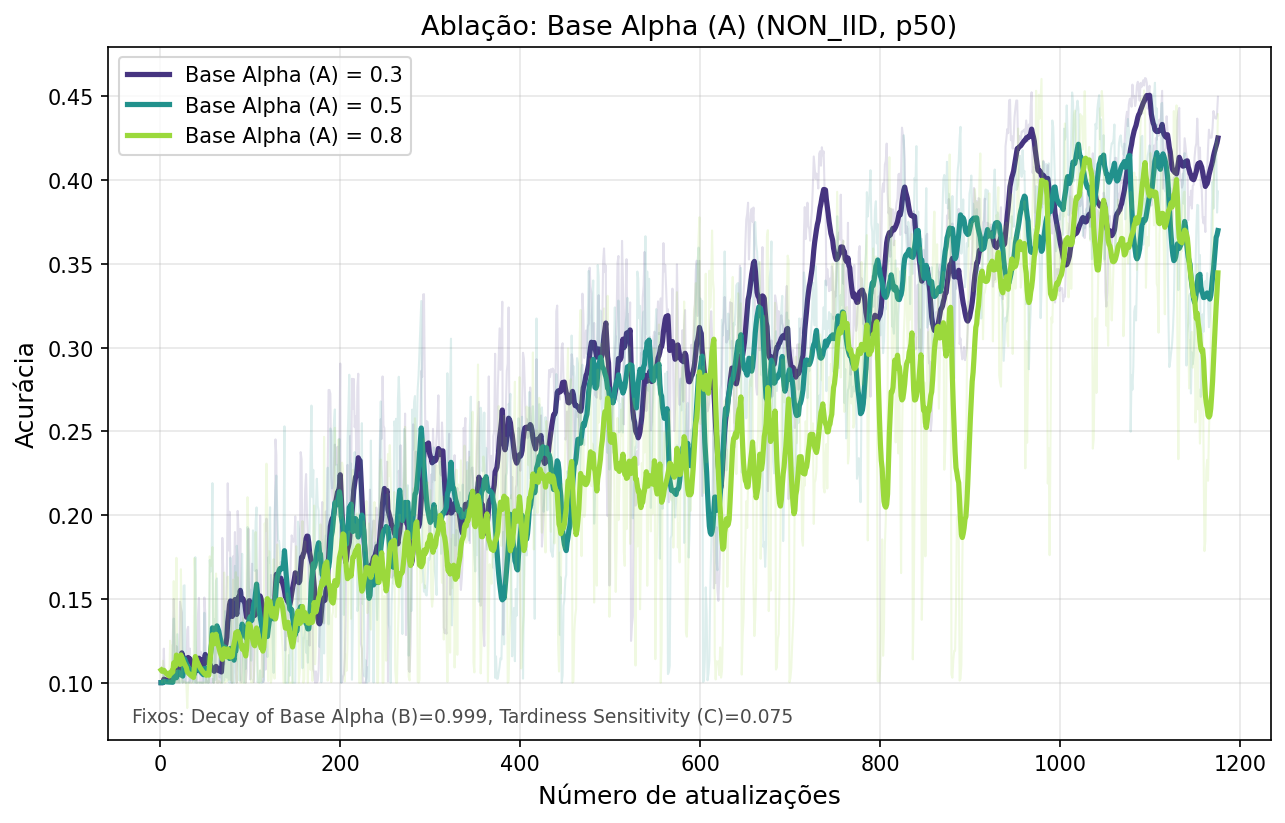
\includegraphics[width=\textwidth]{ablation_base_alpha_non_iid_p50.png}
    \caption{Ablação de $\alpha_0$ — cenário Não-IID.}
\end{figure}

\subsection{Impacto do Decaimento $\delta$}

\begin{table}[H]
\centering
\caption{Impacto de $\delta$ na acurácia. Fixos: $\alpha_0=0{,}8$, $\lambda=0{,}075$.}
\label{tab:beta}
\renewcommand{\arraystretch}{1.25}
\begin{tabular}{ccccc}
\toprule
$\delta$ & IID máx. & IID avg\_last10 & Non-IID máx. & Non-IID avg\_last10 \\
\midrule
0{,}999 & \textbf{0{,}6812} & \textbf{0{,}6800} & \textbf{0{,}4604} & \textbf{0{,}3760} \\
0{,}99  & 0{,}4982          & 0{,}4970          & 0{,}3685          & 0{,}3521          \\
0{,}95  & 0{,}3180          & 0{,}3180          & 0{,}1684          & 0{,}1000          \\
\bottomrule
\end{tabular}
\end{table}

$\delta$ é o parâmetro mais crítico da fórmula. $\delta = 0{,}95$ causa
estagnação em $\approx 32\%$ (IID) e colapso para acurácia aleatória (Non-IID).
Após 100 atualizações: $0{,}95^{100} \approx 0{,}006$ vs.\ $0{,}999^{100} \approx 0{,}905$
.

\begin{figure}[H]
    \centering
    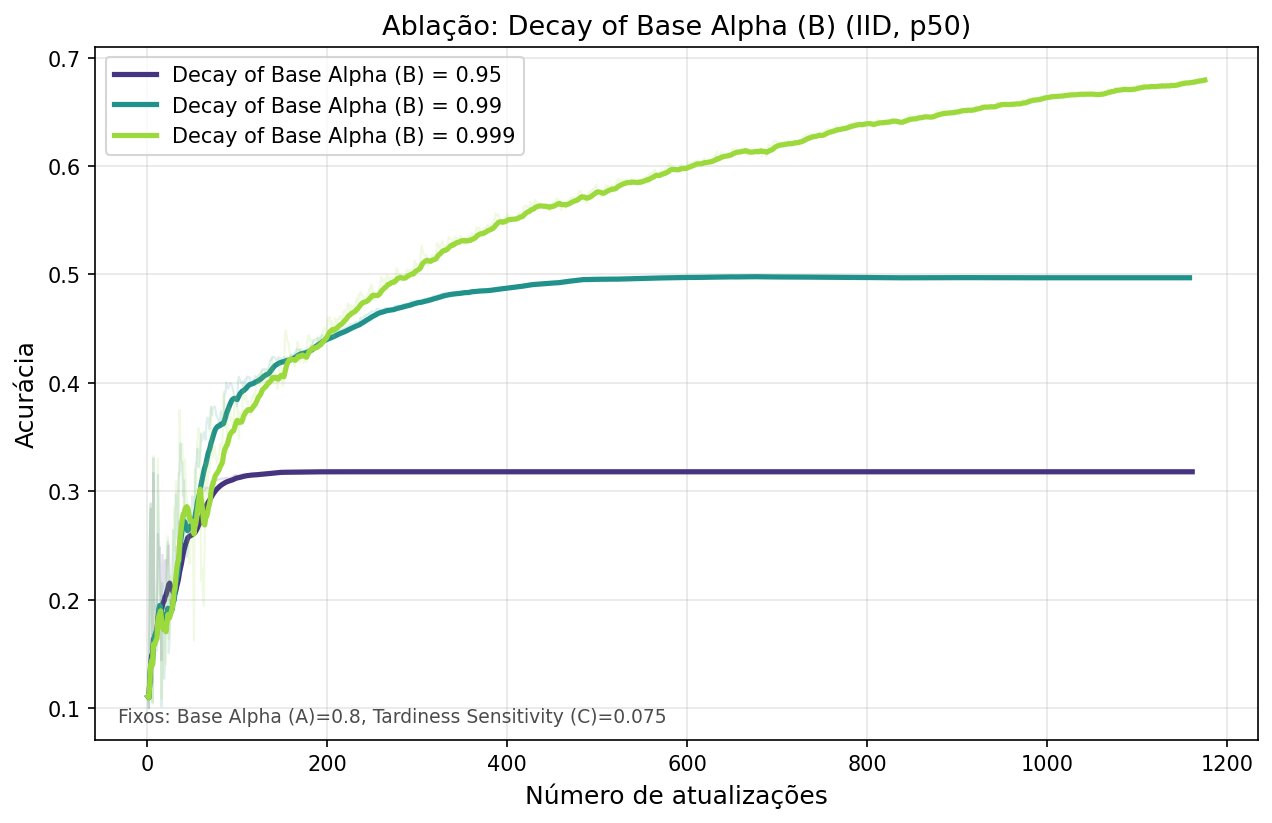
\includegraphics[width=\textwidth]{ablation_decay_iid_p50.png}
    \caption{Ablação de $\delta$ — cenário IID.}
\end{figure}

\begin{figure}[H]
    \centering
    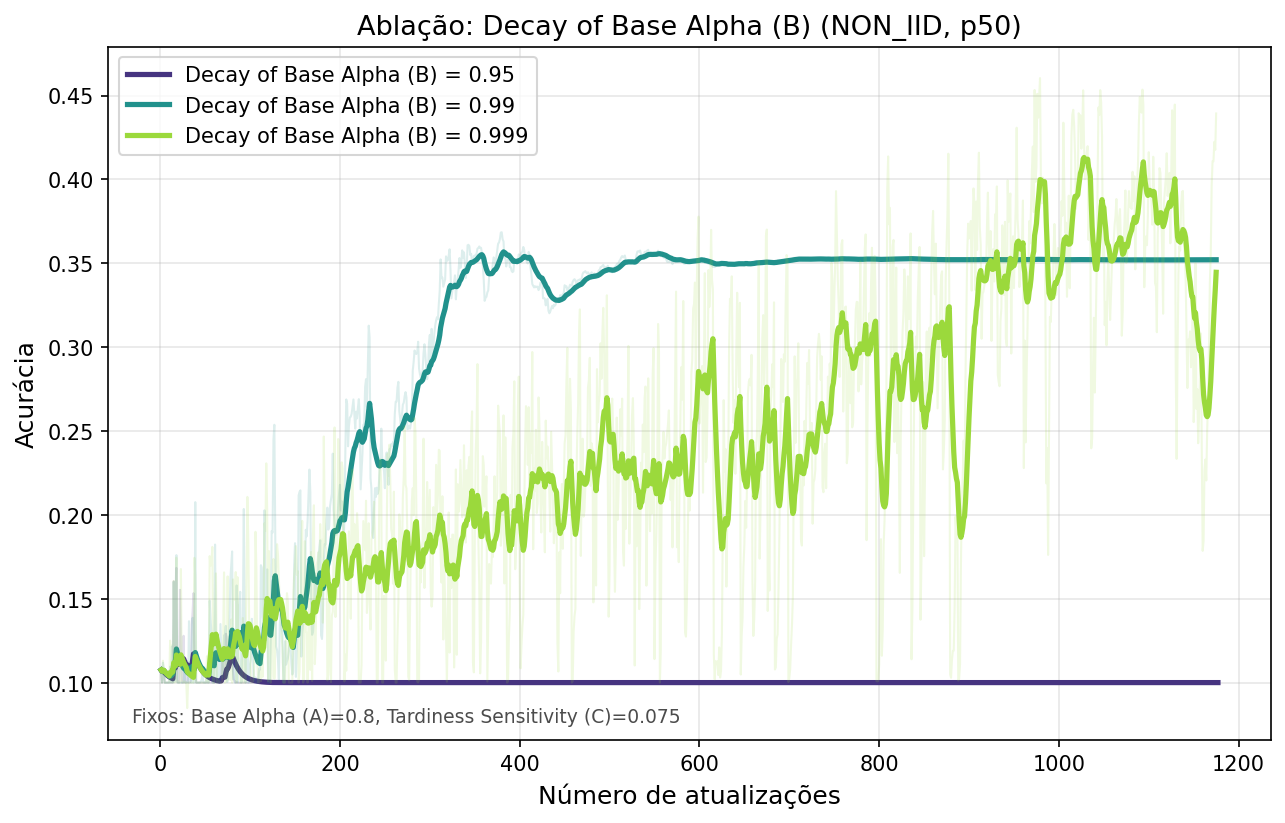
\includegraphics[width=\textwidth]{ablation_decay_non_iid_p50.png}
    \caption{Ablação de $\delta$ — cenário Não-IID.}
\end{figure}

\subsection{Impacto da Sensibilidade ao \textit{Staleness} $\lambda$}

\begin{table}[H]
\centering
\caption{Impacto de $\lambda$ na acurácia. Fixos: $\alpha_0=0{,}8$, $\delta=0{,}999$.}
\label{tab:gamma}
\renewcommand{\arraystretch}{1.25}
\resizebox{\textwidth}{!}{%
\begin{tabular}{cccccc}
\toprule
$\lambda$ & IID máx. & IID avg\_last10 & IID tail\_std & Non-IID máx. & Non-IID avg\_last10 \\
\midrule
0{,}000 & 0{,}6788          & 0{,}6761          & 0{,}0098 & 0{,}2689          & 0{,}1600          \\
0{,}075 & \textbf{0{,}6812} & \textbf{0{,}6800} & 0{,}0066 & \textbf{0{,}4604} & 0{,}3760          \\
0{,}500 & 0{,}6404          & 0{,}6394          & 0{,}0060 & 0{,}4547          & \textbf{0{,}4379} \\
\bottomrule
\end{tabular}}
\end{table}
% Aqui ele faz com que dados mais novos contribuam menos com o modelo global pra evitar de um modelo consolidado ser degradado
Sem penalização ($\lambda = 0$), o modelo colapsa para $\approx 16\%$ em Non-IID. A penalização por \textit{staleness} é estruturalmente necessária
para que a agregação assíncrona funcione em cenários heterogêneos: updates defasados
de clientes com distribuições enviesadas corrompem o modelo global quando incorporados
com peso integral. $\lambda = 0{,}5$ oferece maior estabilidade ($\text{avg\_last10} = 0{,}44$)
ao custo de ligeira redução na velocidade de convergência.

\begin{figure}[H]
    \centering
    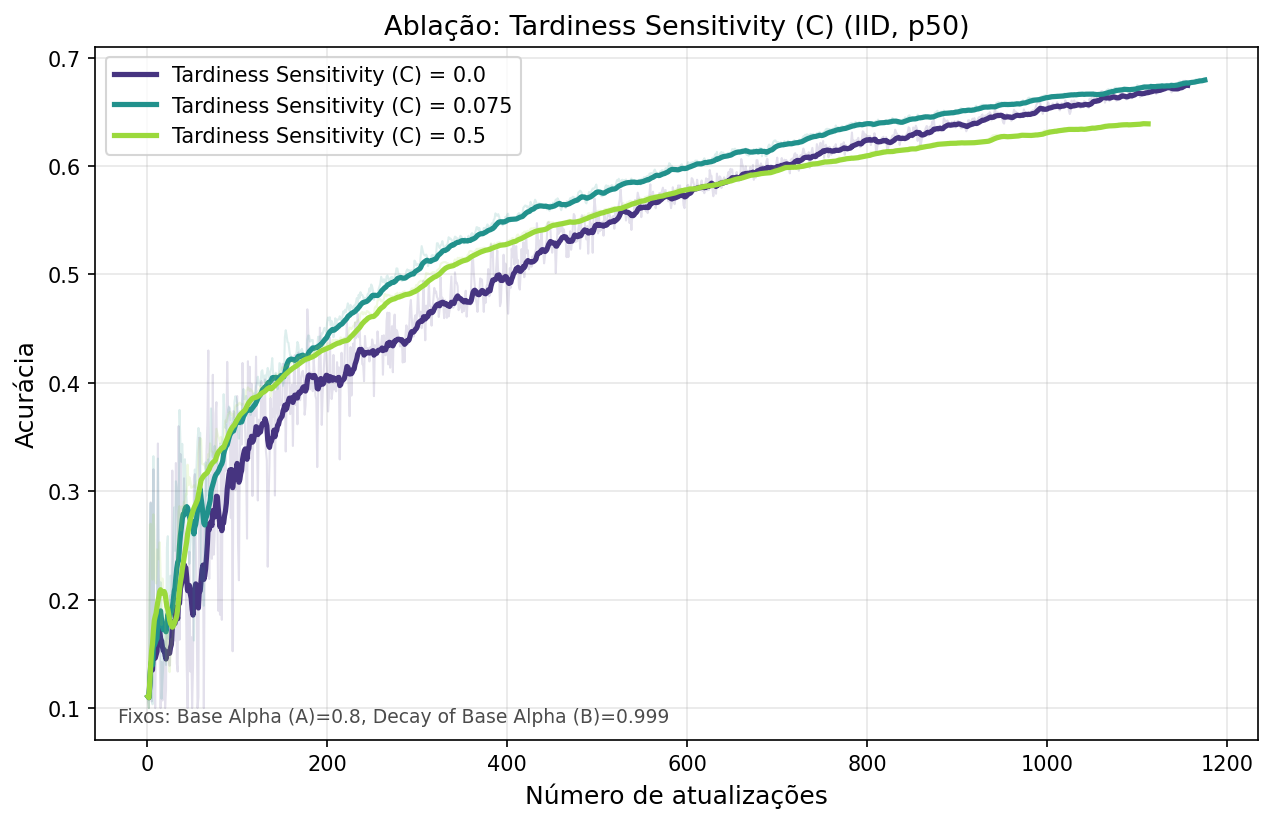
\includegraphics[width=\textwidth]{ablation_tardiness_iid_p50.png}
    \caption{Ablação de $\lambda$ — cenário IID.}
\end{figure}

\begin{figure}[H]
    \centering
    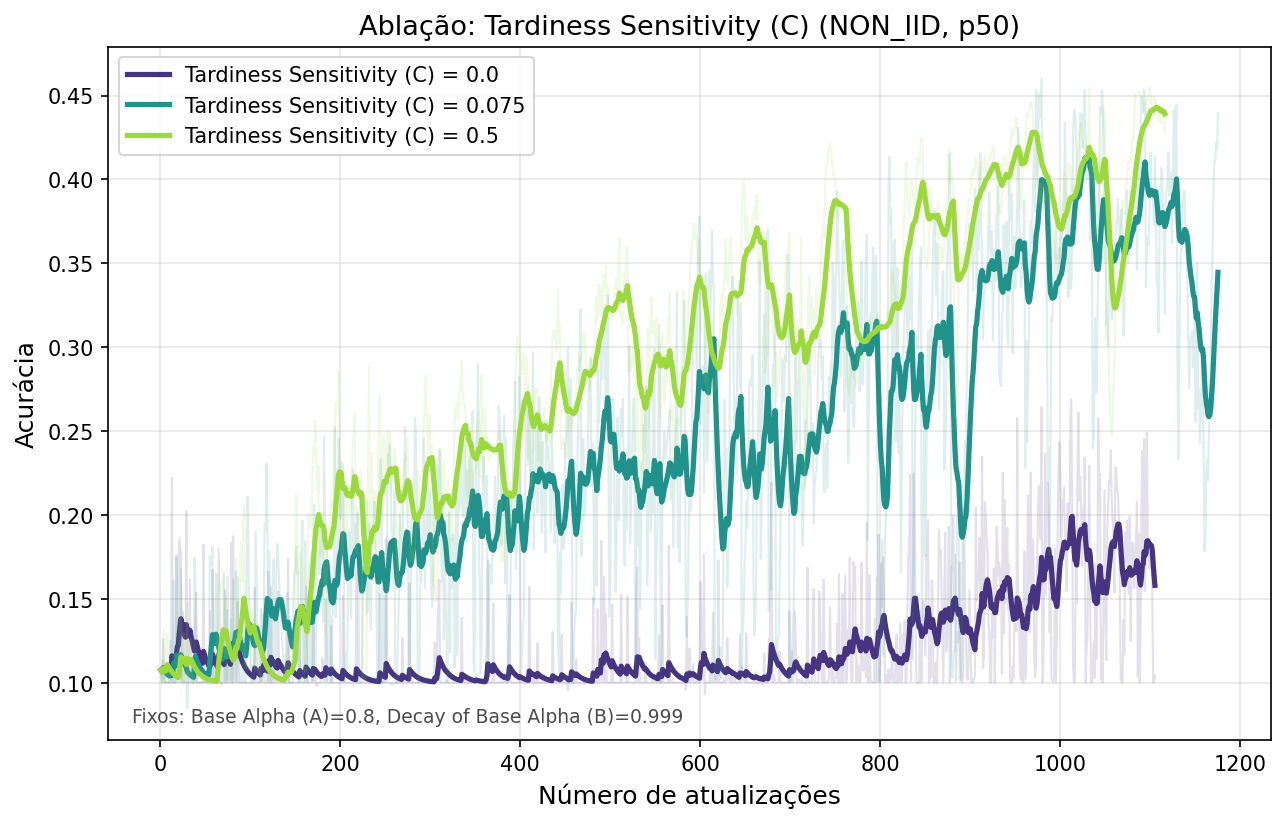
\includegraphics[width=\textwidth]{ablation_tardiness_non_iid_p50.png}
    \caption{Ablação de $\lambda$ — cenário Não-IID.}
\end{figure}

\subsection{Conclusões da Ablação}

\begin{enumerate}
    \item \textbf{$\delta$ é o parâmetro mais sensível}: valores abaixo de $0{,}999$
    causam degradação significativa; $\delta = 0{,}95$ é catastrófico em ambos os
    cenários.
% Basicamente ele pune mais ou menos modelos mais antigos, pra evitar deles jogarem o resultado no lixo
    \item \textbf{$\lambda$ é dispensável em IID, mas indispensável em Non-IID}:
    sem penalização por \textit{staleness}, o sistema simplesmente não funciona em
    cenários heterogêneos — este resultado sugere que $\lambda$ é um pré-requisito
    funcional, não um refinamento cosmético.

    \item \textbf{$\alpha_0$ apresenta trade-off estabilidade vs.\ velocidade}:
    em Non-IID, $\alpha_0 = 0{,}3$ converge mais devagar, mas com metade das
    oscilações de $\alpha_0 = 0{,}8$.

    \item \textbf{A fórmula tripartite é validada}: os três componentes têm papéis
    complementares e não redundantes.

    \item \textbf{Non-IID amplifica todas as sensibilidades}: parâmetros que
    funcionam em IID podem colapsar em Non-IID.
\end{enumerate}

% ─────────────────────────────────────────────
\section{Generalização para Múltiplos Datasets — FL Assíncrono}

Os parâmetros identificados na ablação ($\alpha_0 = 0{,}8$, $\delta = 0{,}999$,
$\lambda = 0{,}075$) foram aplicados sem ajuste fino a quatro datasets distintos,
por $\approx 1\text{h}33\text{min}$ cada.

\subsection{Cenário IID}

\begin{table}[H]
\centering
\caption{Resultados no cenário IID para os quatro datasets.}
\label{tab:iid_datasets}
\renewcommand{\arraystretch}{1.25}
\resizebox{\textwidth}{!}{%
\begin{tabular}{lcccccc}
\toprule
\textbf{Dataset} & \textbf{Aval.} & \textbf{Acurácia Máx.} & \textbf{Média Last10} & \textbf{Tail Std} & \textbf{Conv.\ @90\%} & \textbf{Loss Final} \\
\midrule
MNIST        & 4731 & 0{,}9938 & 0{,}9937 & 0{,}0004 & 3/4731    & 0{,}0191 \\
Fashion MNIST & 3809 & 0{,}9185 & 0{,}9181 & 0{,}0030 & 348/3809  & 0{,}2223 \\
CIFAR-10     & 4645 & 0{,}7362 & 0{,}7349 & 0{,}0108 & 2715/4645 & 0{,}7573 \\
GTSRB        & 2534 & 0{,}9625 & 0{,}9613 & 0{,}0023 & 813/2534  & 0{,}1531 \\
\bottomrule
\end{tabular}}
\end{table}

\subsection{Cenário Não-IID}

\begin{table}[H]
\centering
\caption{Resultados no cenário Não-IID para os quatro datasets.}
\label{tab:noniid_datasets}
\renewcommand{\arraystretch}{1.25}
\resizebox{\textwidth}{!}{%
\begin{tabular}{lcccccc}
\toprule
\textbf{Dataset} & \textbf{Aval.} & \textbf{Acurácia Máx.} & \textbf{Média Last10} & \textbf{Tail Std} & \textbf{Conv.\ @90\%} & \textbf{Loss Final} \\
\midrule
MNIST         & 4828 & 0{,}9859 & 0{,}9837 & 0{,}0033 & 953/4828   & 0{,}0546 \\
Fashion MNIST & 3860 & 0{,}8472 & 0{,}8369 & 0{,}0278 & 1554/3860  & 0{,}4945 \\
CIFAR-10      & 5253 & 0{,}4765 & 0{,}4465 & 0{,}0391 & 4002/5253  & 1{,}4638 \\
GTSRB         & 2633 & 0{,}4899 & 0{,}2374 & 0{,}0759 & 2466/2633  & 2{,}6594 \\
\bottomrule
\end{tabular}}
\end{table}

\subsection{Impacto IID $\to$ Não-IID por Dataset}

\begin{table}[H]
\centering
\caption{Degradação de desempenho ao passar de IID para Não-IID.}
\label{tab:delta_datasets}
\renewcommand{\arraystretch}{1.25}
\begin{tabular}{lccc}
\toprule
\textbf{Dataset} & \textbf{$\Delta$ Acurácia Máx.} & \textbf{$\Delta$ Avg Last10} & \textbf{Razão Tail Std (non/iid)} \\
\midrule
MNIST         & $-0{,}0079$ & $-0{,}0100$ & $8{,}1\times$  \\
Fashion MNIST & $-0{,}0713$ & $-0{,}0812$ & $9{,}3\times$  \\
CIFAR-10      & $-0{,}2597$ & $-0{,}2884$ & $3{,}6\times$  \\
GTSRB         & $-0{,}4726$ & $-0{,}7239$ & $33{,}3\times$ \\
\bottomrule
\end{tabular}
\end{table}

O GTSRB é o dataset mais sensível à heterogeneidade: queda de $47{,}26$ p.p.\ e
instabilidade $33{,}3\times$ maior em Não-IID. Com 43 classes e dados de trânsito
naturalmente desbalanceados por região, reforça a importância de $\lambda$ adaptativo
em datasets multiclasse com alta heterogeneidade natural.

O comportamento observado no CIFAR-10 generaliza para todos os datasets:
convergência consistente em IID, queda de acurácia e maior instabilidade em Não-IID
são padrões universais, e não artefatos do CIFAR-10.

% ─────────────────────────────────────────────
\section{Impacto do \textit{Timeout} — FL Síncrono (CIFAR-10)}

O servidor aguarda os clientes por no máximo $T_p$ segundos por rodada, onde $T_p$
é o percentil $p$ da distribuição empírica de $\Delta t$ (via Monte Carlo),
conforme a Tabela~\ref{tab:timeouts}.

\begin{table}[H]
\centering
\caption{\textit{Timeouts} derivados via simulação de Monte Carlo ($10^6$ realizações).}
\label{tab:timeouts}
\renewcommand{\arraystretch}{1.25}
\begin{tabular}{lcc}
\toprule
\textbf{Configuração} & \textbf{Timeout (s)} & \textbf{Clientes descartados por rodada} \\
\midrule
P25          & 24{,}99 s & 75\% dos clientes lentos \\
P50          & 47{,}45 s & 50\% dos clientes lentos \\
P75          & 69{,}95 s & 25\% dos clientes lentos \\
Sem timeout  & 95{,}00 s & Nenhum                   \\
\bottomrule
\end{tabular}
\end{table}

\paragraph{Geração dos gráficos.}
As curvas suavizadas utilizam EMA com fator $\alpha = 0{,}1$. As bandas de confiança
são calculadas suavizando pela mesma EMA o desvio absoluto entre os dados originais
e a curva suavizada. Os \textit{boxplots} exibem a distribuição bruta por faixas de rodadas.

\subsection{Cenário IID}

\begin{table}[H]
\centering
\caption{Acurácia final e máxima — IID.}
\label{tab:timeout_iid_acc}
\renewcommand{\arraystretch}{1.25}
\begin{tabular}{lccc}
\toprule
\textbf{Configuração} & \textbf{Acurácia R80} & \textbf{Acurácia Máx.} & \textbf{Loss Final} \\
\midrule
P25         & 73{,}7\% & 73{,}8\% & 0{,}7526 \\
P50         & 76{,}6\% & 76{,}7\% & 0{,}6777 \\
P75         & 77{,}7\% & 78{,}1\% & 0{,}6511 \\
Sem timeout & \textbf{79{,}1\%} & \textbf{79{,}2\%} & \textbf{0{,}6311} \\
\bottomrule
\end{tabular}
\end{table}

\begin{table}[H]
\centering
\caption{Tempo de execução e eficiência por hora — IID.}
\label{tab:timeout_iid_time}
\renewcommand{\arraystretch}{1.25}
\resizebox{\textwidth}{!}{%
\begin{tabular}{lcccc}
\toprule
\textbf{Configuração} & \textbf{Tempo/rodada} & \textbf{Tempo total} & \textbf{Ganho vs.\ sem timeout} & \textbf{Acurácia/hora} \\
\midrule
P25         & 28{,}2 s & 37{,}7 min & $-70{,}4\%$ & 117{,}3\%/h \\
P50         & 50{,}7 s & 67{,}6 min & $-48{,}8\%$ &  68{,}0\%/h \\
P75         & 73{,}8 s & 98{,}5 min & $-25{,}4\%$ &  47{,}3\%/h \\
Sem timeout & 99{,}0 s & 132{,}0 min & —           &  35{,}9\%/h \\
\bottomrule
\end{tabular}}
\end{table}

\begin{figure}[H]
    \centering
    
\includegraphics[width=\textwidth]{accuracy_iid.png}
    \caption{Síncrono / IID — curvas de acurácia suavizadas por EMA ($\alpha=0{,}1$),
    comparadas por configuração de \textit{timeout}.}
\end{figure}

\begin{figure}[H]
    \centering
    
\includegraphics[width=\textwidth]{accuracy_bands_iid.png}
    \caption{Síncrono / IID — banda de confiança baseada no desvio absoluto suavizado
    por EMA ($\alpha=0{,}1$).}
\end{figure}

\begin{figure}[H]
    \centering
    
\includegraphics[width=\textwidth]{accuracy_boxplot_iid.png}
    \caption{Síncrono / IID — \textit{boxplot} por faixas de rodadas.}
\end{figure}

\subsection{Cenário Não-IID}

\begin{table}[H]
\centering
\caption{Acurácia final e máxima — Não-IID.}
\label{tab:timeout_noniid_acc}
\renewcommand{\arraystretch}{1.25}
\begin{tabular}{lccc}
\toprule
\textbf{Configuração} & \textbf{Acurácia R80} & \textbf{Acurácia Máx.} & \textbf{Loss Final} \\
\midrule
P25         & 38{,}5\% & 38{,}5\% & 1{,}8796 \\
P50         & 40{,}4\% & 49{,}5\% & 1{,}6215 \\
P75         & 41{,}5\% & 52{,}5\% & 1{,}5789 \\
Sem timeout & \textbf{50{,}6\%} & \textbf{51{,}4\%} & \textbf{1{,}3255} \\
\bottomrule
\end{tabular}
\end{table}

\begin{table}[H]
\centering
\caption{Estabilidade nas últimas 10 rodadas — Não-IID.}
\label{tab:timeout_noniid_stability}
\renewcommand{\arraystretch}{1.25}
\begin{tabular}{lccc}
\toprule
\textbf{Configuração} & \textbf{Desvio Padrão} & \textbf{Mín.} & \textbf{Máx.} \\
\midrule
P25         & 0{,}0559 & 20{,}7\% & 38{,}5\% \\
P50         & 0{,}0640 & 27{,}9\% & 49{,}5\% \\
P75         & 0{,}0644 & 32{,}0\% & 52{,}5\% \\
Sem timeout & \textbf{0{,}0374} & \textbf{40{,}4\%} & \textbf{51{,}4\%} \\
\bottomrule
\end{tabular}
\end{table}

\begin{figure}[H]
    \centering
    
\includegraphics[width=\textwidth]{accuracy_non_iid.png}
    \caption{Síncrono / Não-IID — curvas de acurácia suavizadas por EMA ($\alpha=0{,}1$),
    comparadas por configuração de \textit{timeout}.}
\end{figure}

\begin{figure}[H]
    \centering
    
\includegraphics[width=\textwidth]{accuracy_bands_non_iid.png}
    \caption{Síncrono / Não-IID — banda de confiança baseada no desvio absoluto suavizado
    por EMA ($\alpha=0{,}1$).}
\end{figure}

\begin{figure}[H]
    \centering
    
\includegraphics[width=\textwidth]{accuracy_boxplot_non_iid.png}
    \caption{Síncrono / Não-IID — \textit{boxplot} por faixas de rodadas.}
\end{figure}

\subsection{Conclusões}

\begin{enumerate}
    \item \textbf{O \textit{timeout} tem impacto significativo e mensurável} em acurácia
    e tempo de treinamento no cenário síncrono com CIFAR-10.

    \item \textbf{Em IID}, o impacto é moderado: mesmo o timeout mais agressivo (P25)
    converge para $73{,}7\%$, uma redução de $5{,}4$ p.p.\ em relação ao sem-timeout,
    mas com $3{,}5\times$ menos tempo total. Em termos de acurácia por hora, P25
    ($117{,}3\%$/h) supera amplamente o sem-timeout ($35{,}9\%$/h).

    \item \textbf{Em Não-IID}, o impacto é grave: P25 nunca atinge $40\%$ de acurácia,
    e o sem-timeout é o único que ultrapassa $50\%$. A diferença de $12{,}1$ p.p.\
    entre P25 e sem-timeout (vs.\ $5{,}4$ p.p.\ no IID) indica que excluir clientes
    lentos prejudica a generalização em cenários heterogêneos, pois esses clientes
    podem possuir dados sub-representados.

    \item \textbf{Para cenários dinâmicos} (e.g., dispositivos móveis), o timeout
    deve ser escolhido com cuidado. Um timeout muito curto pode excluir sistematicamente
    clientes com dados raros, amplificando o dano em Non-IID.

    \item \textbf{A simulação de Monte Carlo} para calibrar o timeout via percentis
    da distribuição de latência mostrou-se uma abordagem controlada e principiada
    para explorar esse espaço de parâmetros.
\end{enumerate}

\end{document}
